\entry{Semana del 19/05/2025}

\section{Lunes 19/05/2025}
La idea es volver a probar el Lockin el día de hoy. Según dice el manual, el modo A que estuvismos usando es single-ended. Tanto la configuración Ground como float conectan a Tierra, pero la primera con una resistencia de 10 $\Omega$ y la segunda internamente con una resistencia de 10 k$\Omega$. Lo que queremos hacer nosotros debería utilizar dos entradas con el modo diferencial A-B. Se supone que el float es para conectar la Tierra a la de los equipos, mientras que Ground es para usar la propia del Lock-in. 

Respecto al AC/DC, se supone que cualquier cosa con más de 136 mHz debería usar el acoplamiento AC, así que eso estaba bien.

\subsection*{Resumen rápido}
\begin{itemize}
	\item Aún en modo diferencial el lock-in de la vez pasada no aprecía funcionar correctamente (o como era esperado). Daba bien intercambiar cables (salto de 180°, no 90°) pero no poner el capacitor a tierra.
	\item El otro lock-in (con el sticker) pasaba lo mismo. 
	\item Cambiamos los tres componentes y empezó a funcionar (en las cuatro configuraciones daba 90° en la resonancia). Testeamos con el multímetro los anteriores y los valores daban bien así que no sabemos porqué pasaba eso. No volvimos a probar el Lock-in anterior.
	\item Hicimos pruebas forzando el agua y las calibraciones con y sin Photo-Flo y con sal. 
	\item Calculamos las frecuencias características de la caja con las dimensiones de la misma, para comparar con las que salían de timear el tiempo entre medición y medición del lock-in. % $ a y p
\end{itemize}

\section{Frecuencia de Sampleo.}
Para tomar las mediciones de la fase con el Lock-in usamos el código de Diego Shalom, con un loop que tome mediciones, y el tiempo entre sampleos se midio con el módulo \textit{Time} de Python:

\begin{lstlisting}
measures = []
intervalos = []
	
t0 = time.time()
	
for i in range(200):
	t1 = time.time()
	phi = lock.get_medicion(isXY=False)[1]
	measures.append(phi)
	t2 = time.time()
	intervalos.append(t2 - t1)  
	t0 = t2
\end{lstlisting}

Y la función que toma la medición en cuestión es:

\begin{lstlisting}
def get_medicion(self,isXY = True):
	orden = "SNAP? "
	if isXY:
	self._lockin.write("DDEF 1,0") #Canal 1, XY
	orden += "1, 2" #SNAP? 1,2
	else:
	self._lockin.write("DDEF 1,1") #Canal 1, RTheta
	orden += "3, 4" #SNAP? 3, 4
	return self._lockin.query_ascii_values(orden, separator=",")
\end{lstlisting}	
	
Los resultados fueron los que se ven más abajo, con $T_s = (0.039 \pm 0.004)$ s, o lo que es equivalente, $f=25.6$ S/s.

\begin{figure}[th!]
	\centering
	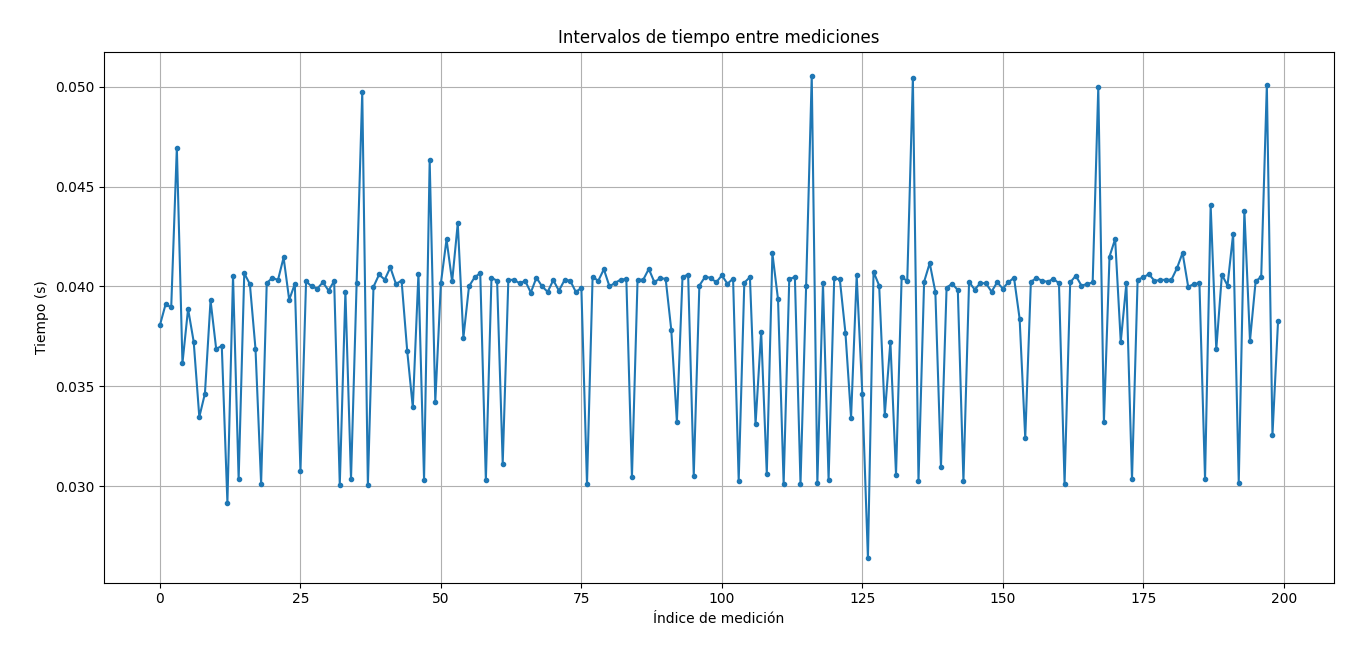
\includegraphics[width=0.87\linewidth]{Figures/19_05_2025/Frecuencia_de_sampleo}
	\caption{Tiempo entre mediciones consecutivas del Lock-in.}
	\label{fig:frecuenciadesampleo}
\end{figure}


\section{Comportamiento inicial - Agua destilada.}
Empezamos analizando el funcionamiento del sensor en agua destilada (la del filtro del Labo). Para esto usamos una pecera de vidrio que encontramos arriba en Labo 4/5. Un detalle importante es que tenía brillantina dorada depositada en el fondo, que intentamos limpiar pero estaba pegada y recién se empezó a resuspender en el agua luego de un rato. 

Las dimensiones del tanque fueron, medidas desde afuera con un metro: 
\begin{itemize}
	\item Largo: 22.0 cm.
	\item Ancho: 11.1 cm.
	\item Alto del agua: 5 cm.
	\item Grosor de paredes y piso: 3 mm.
\end{itemize}

Las dimensiones calculadas en consecuencia (restando las paredes y piso): 
\begin{itemize}
	\item Largo: 21.4 cm.
	\item Ancho: 10.5 cm.
	\item Alto del agua: 4.7 cm.
\end{itemize}

La configuración del RLC solo sin sensor fue de 78.55 kHz para fase -89.87° y 2.148 mV, en $\tau=10$ ms y 6 dB. Siempre usamos los 2 filtros (línea de 50 Hz y 2 x línea de 100 Hz, para un total de 150 Hz). 

Lo primero que hicimos fue buscar la frecuencia de resonancia del sistema con el sensor sumergido. Al conectarlo bajó un poco la fase. Ajustamos la frecuencia a 81.68 kHz para que la fase fuese exactamente -90°. La amplitud pasó a ser de 1.823 mV, acá dudo de si tal vez nos paramos en algo que no era la resonancia, aunque terminó funcionando en cualquier caso.

Luego empezamos a sacudir la pecera para ver si veíamos reflejadas las oscilaciones del agua en la fase que medía el Lock-in. Acá nos dimos cuenta de un par de cosas:
\begin{itemize}
	\item Al tocar la pecera para sacudir el agua se daba un salto en la fase, lo que creemos que se debe a un cambio de Tierra del fluido. Haciendo más adelante pruebas de continuidad con el multímetro vimos que el alambre de acero sí estaba a Tierra como queríamos pero al probar el agua no sonaba que fuese continuo (incluso volviendo el agua muy conductora al agregar sal). 
	\item Al tocar el tornillo micrométrico pasaba lo mismo, se daba un salto en la fase.
	\item Las oscilaciones se veían bien pero con bastante ruido. Acá decidimos empezar a variar el tiempo de integración $\tau$. Ellos (\cite{gordillozavaletaNonpropagatingHydrodynamicSolitons2012} usaban $\tau=10$ ms). 
\end{itemize}

En la Figura se nota (en amarillo) cómo solo al estar en reposo el agua y tocar y dejar de tocar la pecera se dan saltos en la fase, y mientras se fuerza (en azul) pasa lo mismo. 

\begin{figure}[!ht]
	\centering
	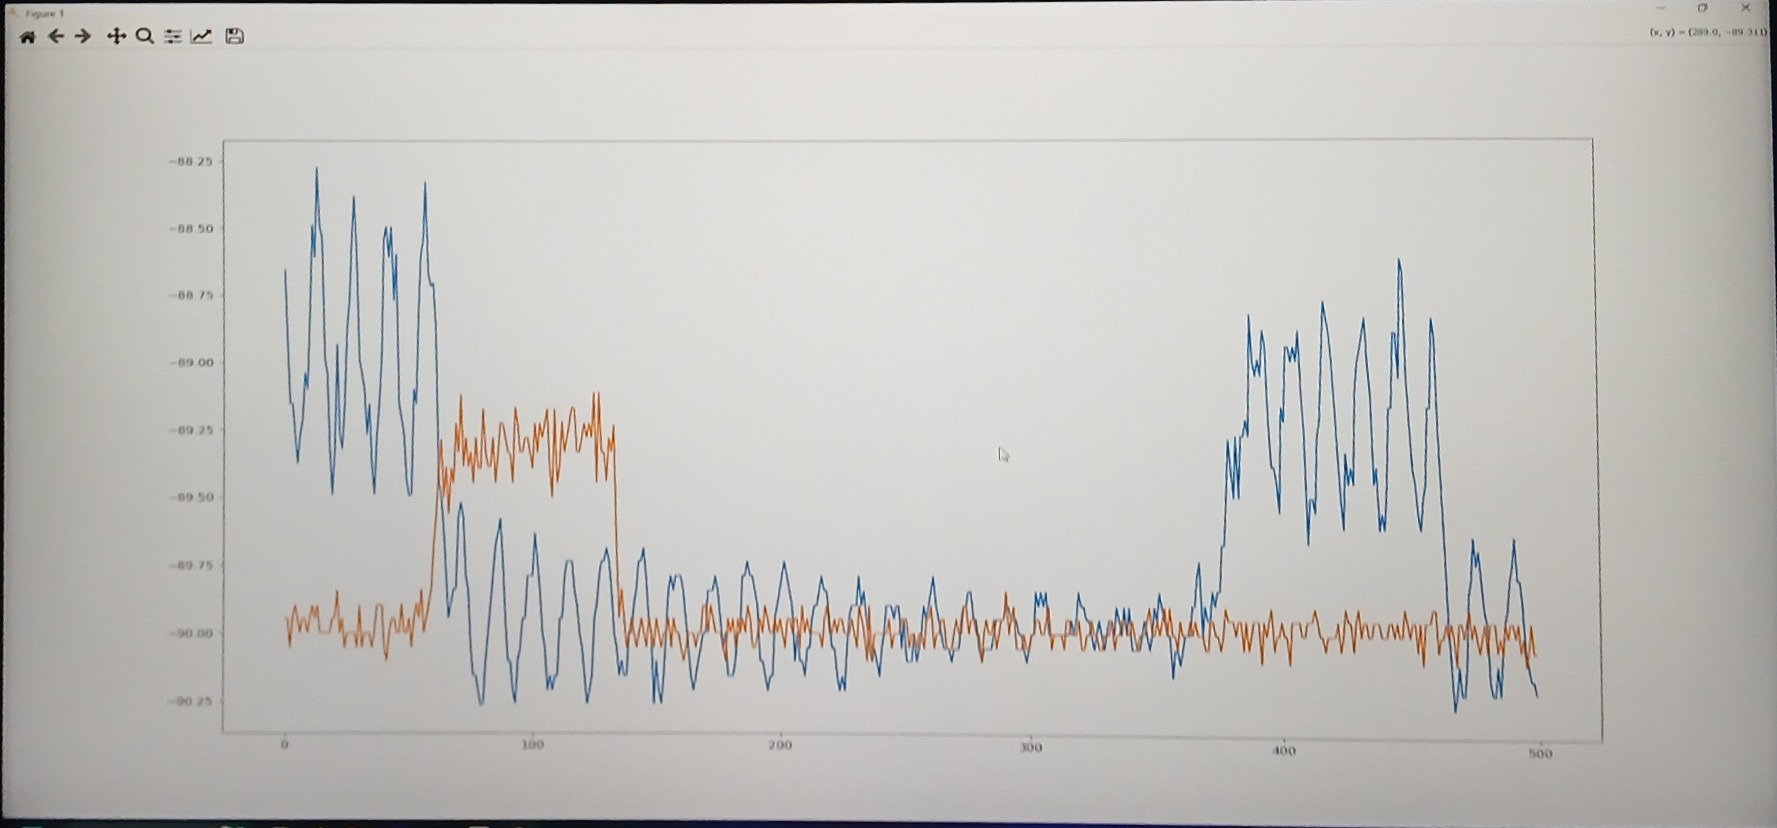
\includegraphics[width=0.957\linewidth]{Figures/19_05_2025/Saltos_de_fase_al_tocar}
	\caption{En Azul forzado y después se suelta la pecera y se vuelve a tocar hacia el final. En amarillo el agua en reposo y de repente se toca por un tiempo la pecera sin moverla.}
	\label{fig:saltosdefasealtocar}
\end{figure}

Después tratamos de reducir el ruido variando el tiempo de integración, como se ve en la Figura de abajo. 

\begin{figure}[!ht]
	\centering
	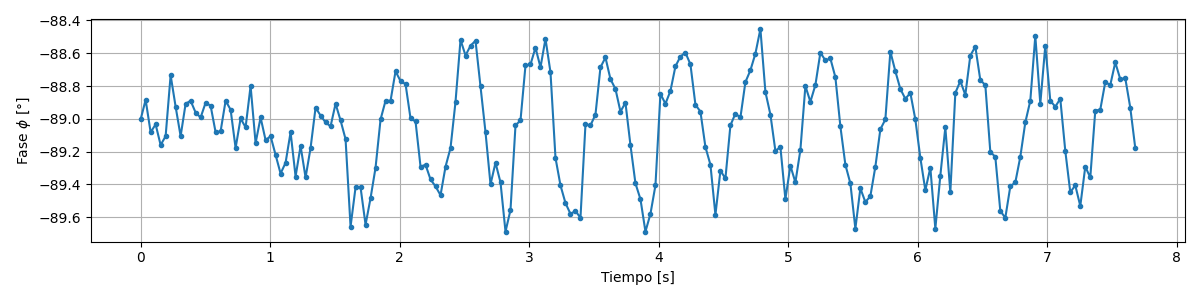
\includegraphics[width=0.8597\linewidth]{Figures/19_05_2025/3ms}
	
	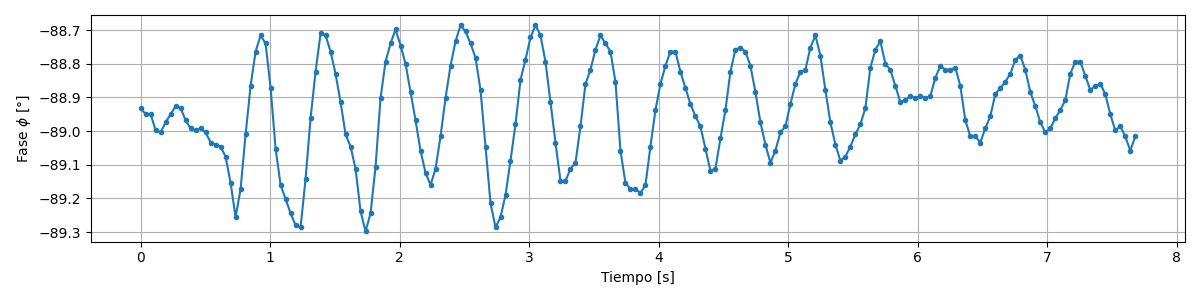
\includegraphics[width=0.8597\linewidth]{Figures/19_05_2025/30ms}
	
	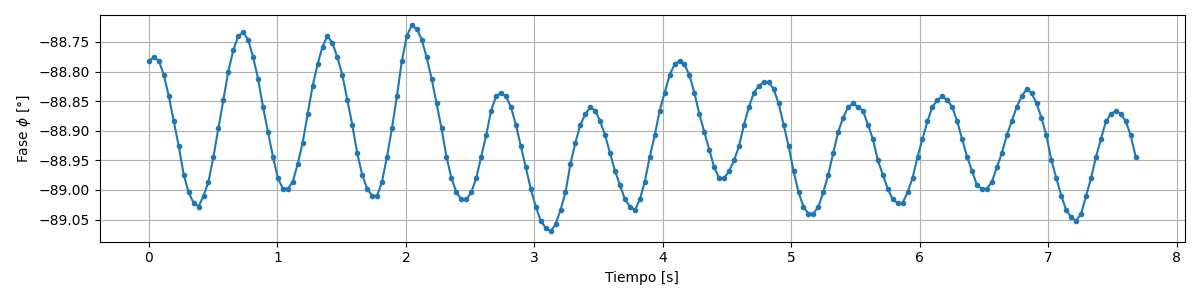
\includegraphics[width=0.8597\linewidth]{Figures/19_05_2025/100ms_24dB}
	\caption{De arriba hacia abajo aumenta la constante de integración en un forzado que deace. Son $\tau=3$ ms, 30 ms y 100 ms. Notar cómo al aumentarlo disminuye el ruido y se suaviza la señal.}
	\label{fig:taus_variables}
\end{figure}


De acá en adelante nos quedamos con $\tau = 100$ ms para el resto de las pruebas. 

\section{Curva de calibración - Agua destilada.}
Algo importante es que las calibraciones se hicieron sin tocar nada cerca del sensor, pero que las mediciones algunas se hicieron tocando la pecera donde se producía un salto en el valor medio de la fase. Por ejemplo al tocar el tornillo pasaba de ser -90° a -89.88°. 
 
Arrancamos con el tornillo en 10 y la frecuencia de resonancia ajustada en 81.25 para que la fase fuese -90°. Fuimos cambiando en ambos sentido el tornillo de a 0.5. Acá paramos cuando tres valores dieron lo mismo ya que parecía que el sensor ya saturaba como mostraban las "simulaciones". 

\begin{figure}[th!]
	\centering
	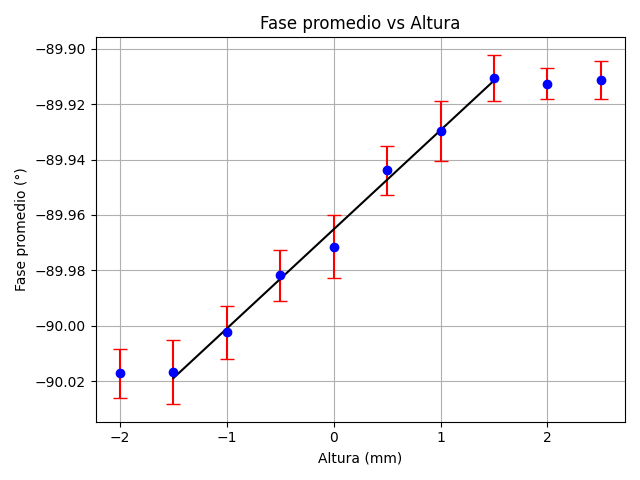
\includegraphics[width=0.87\linewidth]{Figures/19_05_2025/Calibraci+on_agua_sola}
	\caption{Calibración para agua destilada sola, con el ajuste lineal en la zona central.}
	\label{fig:calibracionaguasola}
\end{figure}

% LinregressResult(slope=0.03577714285714352, intercept=-89.96518714285712, rvalue=0.9966758396308251, pvalue=1.2214759716576665e-06, stderr=0.001307860692826204, intercept_stderr=0.001307860692826204)
Los parámetros que obtuvimos de este ajuste lineal son: $R^2=0.99668$,	$m = (0.036 \pm 0.001)\; mm/ ^\circ$,	$b = (-89.96 \pm 0.001)\; mm$ para un ajuste lineal de la forma $f(x)=mx+b$. % ° 

\begin{figure}[th!]
	\centering
	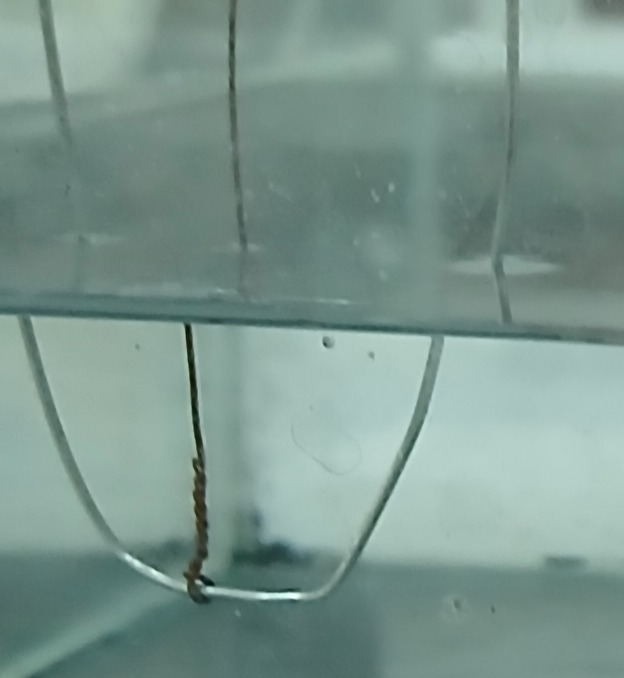
\includegraphics[width=0.2357\linewidth]{Figures/19_05_2025/Rulos}
	\caption{Zoom del rulo donde toca el alambre de cobre con el de acero, se tuvo cuidado de que no llegase a tocar la superficie libre.}
	\label{fig:rulos}
\end{figure}


\section{Curva de calibración - Agua destilada con PhtoFlo.}
Después de agregar una cucharadita blanca con PhotoFlo se repitió la calibración. Ahora nos dimos cuenta de que pasando los dos puntos donde parecía que saturaba seguía moviéndose de forma más o menos lineal, así que seguimos avanzando con el tornillo en ambo sentidos. Además al forzarlo no parecía saturar muy rápido, daban fases por fuera de lo que parecía el rango lineal anterior.

\begin{figure}[th!]
	\centering
	\includegraphics[width=0.87\linewidth]{Figures/19_05_2025/Validación_con_PhotFlo}
	\caption{Calibración para agua destilada con PhotoFlo. Se muestra el ahuste lineal y residuos.}
	\label{fig:validacionconphotflo}
\end{figure}


Acá los resultados del ajuste fueron: $R^2=0.99338$,	$\chi^2=0.91502$,	$m = (0.0265 \pm 0.0003)\; mm/^\circ$,	$b = (-90.011 \pm 0.002)\; mm$. Notamos que en ambos casos da muy lineal y con un slope similar, aunque ligeramente mayor en el caso sin PhotoFlo, donde debería mojarse el alambre de cobre. % $ %  ° % v % intercept


% $R^2=0.99338$,	$ch^2=0.91502$,	$m = (0.0265 \pm 0.0003)\; mm/°$,	$b = (-90.276 \pm 0.004)\; mm$

Importante: en la última altura (con el sensor lo más alto posible) tuvimos cuidado de no llegar a los rulos que tiene donde se conecta con el alambre de acero (que por el esmalte parece que se pegaron), pero inicialmente dio un valor de -89.12256° muy lejos de la tendencia, y resulta que había una brillantina tocando el sesnor en ese momento, después de sacarla repetimos la medición y dio coherente con la tendencia, así que pensamos que fue eso.


\section{Validación del sensor - Agua destilada con PhotoFlo.}
Para saber si lo que estaba midiendo el sensor era coherente o si eran cosas con histéresis/Retraso entre otras cosas tomamos la medición del forzado y calculamos la FFT, para comparar con las frecuencias naturales que surgen de las dimensiones de la pecera:

\begin{equation}
	2\pi f_{nm} = \sqrt{\left(gk_{nm}+\frac{\sigma}{\rho}k_{nm}^3\right)\tanh(k_{nm}d)}
\end{equation}

Con los $k_{nm}^2=k_{xn}^2+k_{ym}^2$ y $k_{(x,y)(n,m)} = \pi*(n,m)/(w,h)$ Siendo $(w,h)$ el largo y ancho (acá $w$ es la longitud mayor). Además $\sigma=0.072$ acá lo tomamos como $0.040$ por haber agregado el PhotoFlo, aunque esto último no cambiaba especialmente las frecuencias naturales en el rango de Gravedad (hasta tipo 10 Hz). % np. 

\begin{figure}[!ht]
	\centering
	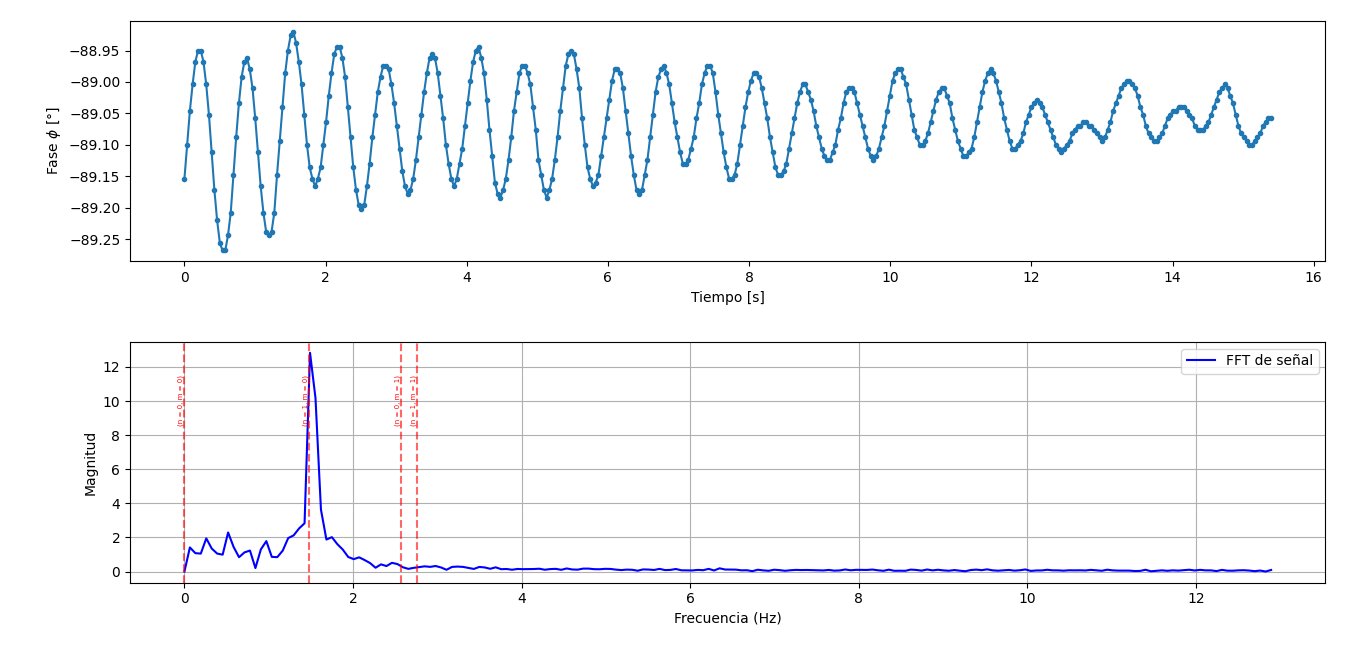
\includegraphics[width=0.87\linewidth]{Figures/19_05_2025/Caracterización_validación_con_PhotoFlo}
	\caption{FFT de las oscilaciones de agua destilada con PhotoFlo, y en rojo marcadas verticalemente las primeras frecuencias naturales de la pecera. oincide bastante bien el primer pico con el primer modo longitudinal (la dirección más larga, que es en la que lo estábamos forzando).}
	\label{fig:caracterizacionvalidacionconphotoflo}
\end{figure}

Se nota que la frecuencia más excitada es la primera longitudinal, en la dirección que estábamos forzando al aistema, como era de esperarse. Estaría bueno forzar en la otra dirección o en diagonal o algo más general.



\section{Comportamiento - Agua con sal y PhotFlo.}
Para terminar agregamos una cucharada de sal al agua con PhotFlo para tratar de aumentar la conductividad. Entonces cambió la fase de equilibrio de -90° a -91.23°, con lo cual ajustamos la frecuencia de resonancia a 78.52 kHz para volver a -90° y medimos el decaimiento del forzado. Sin embargo como se ve abajo no parece funcionar correctamente, casi que es puro ruido. En \cite{gordillozavaletaNonpropagatingHydrodynamicSolitons2012} usaban de 10 a 30 ppm, nosotros una cucharada que supongo sería bastante más. Tal vez habría que replicar la mezcla y medir la conductividad de alguna manera. 

\begin{figure}[th!]
	\centering
	\includegraphics[width=0.87\linewidth]{Figures/19_05_2025/Agua_con_sal_relajación}
	\caption{Fases durante la relajación del forzado del agua con sal.} %  .  
	\label{fig:aguaconsalrelajacion}
\end{figure}


 







